% https://pxl-digital.pxl.be/page/care-athon-2020#

% TODO: screenshots

De tweedaagse hackathon werd gehouden op de Corda Campus in gebouw 3 bij Cegeka. We werden hier ontvangen door Tristan Fransen en Francis Vos, hij gaf ons een korte introductie. Daarna maakte we kennis met de twee vertegenwoordigers van Ambulance Wens en Arno Barzan, de PXL\hyp{}begeleider. Arno Barzan gaf ons meer specifieke uitleg over hoe en wat er precies gerealiseerd moest worden. Mijn willekeurig ingedeelde team bestond uit vier studenten van applicatie\hyp{}ontwikkeling en één systeem\hyp{} en netwerkbeheerder.

Ik heb gekozen voor de uitdaging van Ambulance Wens, dit is een vzw die zich inzet voor mensen met een ongeneeslijke ziekte, die niet mobiel zijn en voelen dat het afscheid nabij komt. Ze zorgen dat deze mensen hun laatste wens nog in vervulling kunnen brengen met de medische ondersteuning die ze nodig hebben. Zo kunnen ze nog eens met volle teugen genieten van het leven en zich haast opnieuw goed voelen in hun vel.

Omdat de interne organisatie en het tentoonstellen van wensen nog ouderwets en stroef verliep, kregen wij de opdracht om een mobiele applicatie te ontwerpen voor de vzw. Zodat hierop niet alleen de pati\"enten een wens konden kiezen, maar dat er achterliggend ook verplegers en vrijwilligers konden deelnemen aan deze wensen. De nadruk lag dus vooral op de gebruiksvriendelijkheid en de consistentie van de applicatie.

Toen de hackathon daadwerkelijk van start ging, zijn we begonnen met iedereen in ons team een taak te geven. Zo moesten één student zich vooral focussen op het maken van de mock\hyp{}ups, twee studenten onderzoek doen naar realiseerbaarheid en restricties van buitenaf en de overige twee begonnen de applicatie te ontwikkelen. Zo kreeg ik de taak om de applicatie te ontwikkelen, maar ik hielp ook met beslissingen te nemen in verband met de mock\hyp{}ups. De applicatie werd geschreven voor Android in Android Studio met Java als programmeertaal. De mock\hyp{}ups werden uitgewerkt in de webapplicatie van Marvel.

Tegen het einde van de eerste dag zijn we als team tot besluit gekomen dat we geen volledige uitgewerkte applicatie konden presenteren in de gegeven tijd. Daarom zijn we de tweede dag ons meer gaan focussen op het afwerken en verfijnen van de mock\hyp{}ups, omdat we het belangrijker vonden om ons idee naar voren te brengen dan een half afgewerkt product. Dus vanaf toen zijn we met drie studenten gaan werken aan de mock\hyp{}ups en de andere twee studenten verder onderzoek naar elementen als server hosting en GDPR\hyp{}wetgeving.

\begin{figure}[!h]
  \centering
  \begin{subfigure}[h]{0.3\textwidth}
    \centering
    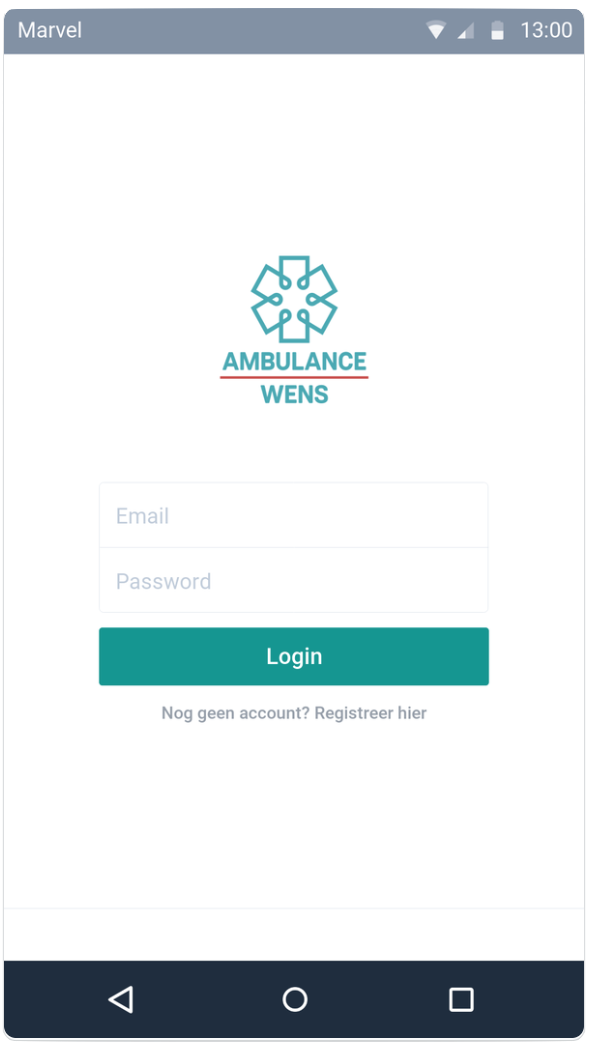
\includegraphics[width=0.76\textwidth]{care-athon/login.png}
  \end{subfigure}
  \begin{subfigure}[h]{0.3\textwidth}
    \centering
    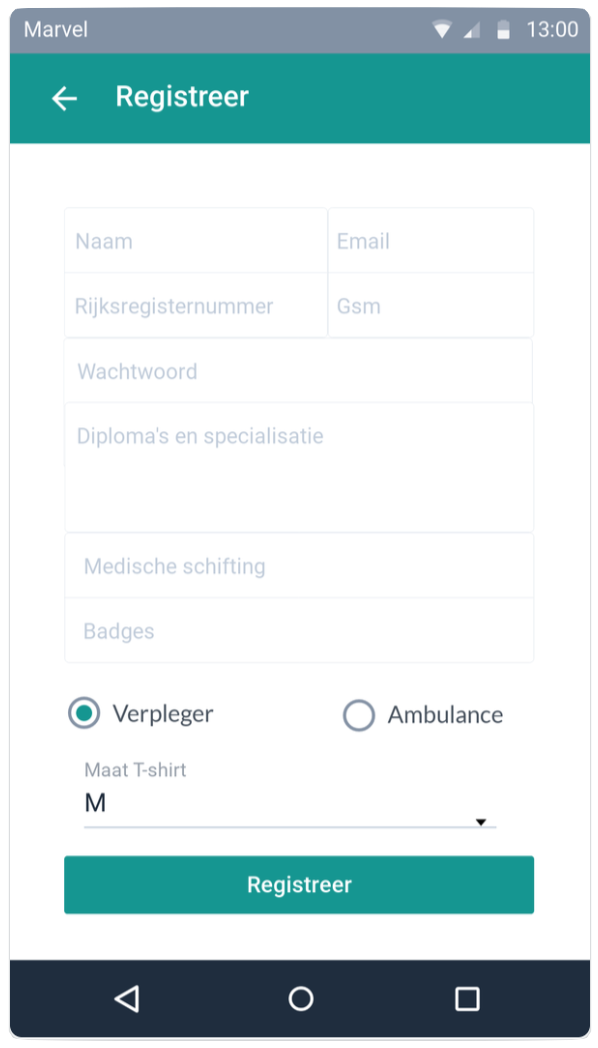
\includegraphics[width=0.76\textwidth]{care-athon/registreer.png}
  \end{subfigure}
  \begin{subfigure}[h]{0.3\textwidth}
    \centering
    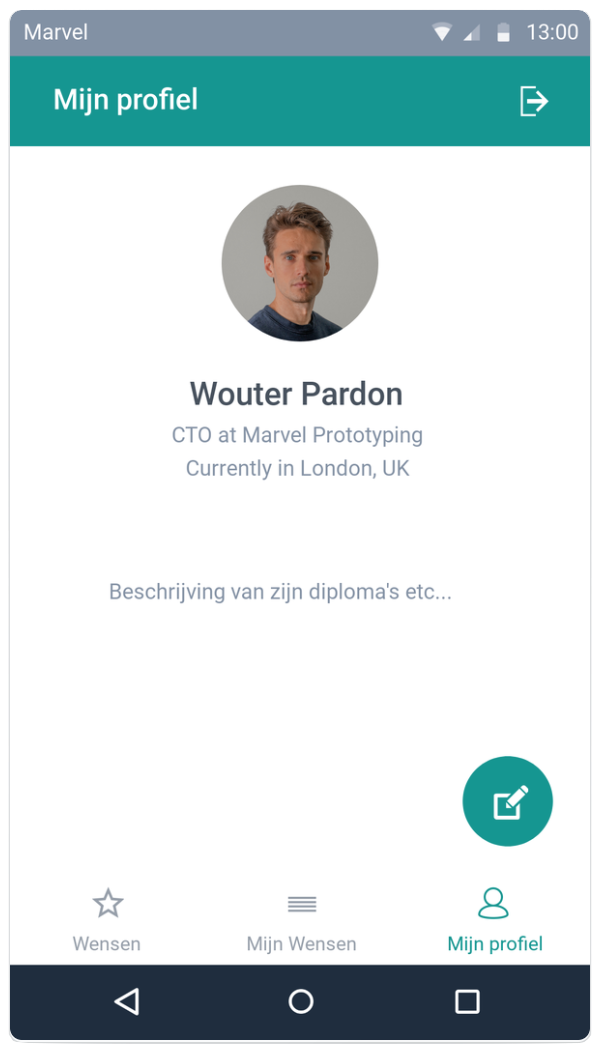
\includegraphics[width=0.76\textwidth]{care-athon/profiel.png}
  \end{subfigure}
\end{figure}

We konden regelmatig feedback gaan vragen aan Arno Barzan en aan de twee vertegenwoordigers van Ambulance Wens, dit gaf ons meer inspiratie en duidelijkheid om de applicatie zo goed mogelijk te ontwerpen aan hun vereisten. Zo wisten we welke informatie van pati\"enten, vrijwilligers en verplegers ze nodig hadden in hun applicatie. Maar ook hoe we het ontwerp in hun stijl konden verwerken.

Uiteindelijk moetsten we ook een presentatie maken die aan het eind van de hackathon gepresenteerd ging worden voor alle studenten van alle uitdagingen. Onze presentatie was een demo van de applicatie aan de hand van de mock\hyp{}ups. Maar omdat we ook ons onderzoek aan Ambulance Wens wouden geven hadden we een document gemaakt met alle informatie die we hadden gevonden en onze mening over bepaalde beslissingen die ze moesten maken.

Aan het einde van de hackathon kwamen iedereen die hieraan deelnam samen in een aula om te luisteren naar verschillende sprekers. Daarna waren de presentaties van alle teams, na dezen presentaties werden de winnaars van elke uitdaging bekend gemaakt en zij ontvingen een prijs afhankelijk van hun gekozen uitdaging.

Ik heb veel praktische zaken bijgeleerd van deze hackathon, zoals het maken van mock\hyp{}ups en het ontwikkelen van een applicatie met zeer specifieke restricties. Voordien had ik nog nooit zo een harde nadruk gelegd op het maken van mock\hyp{}ups, dit leerde ik van de student applicatie\hyp{}ontwikkeling met full\hyp{}stack development als keuzetraject. Maar ook het nadenken over hoe de applicatie er uit moet zien als er zoveel eisen en restricties bij komen kijken heeft mij anders doen denken over bepaalde ontwerp zaken en dus uiteindelijk ook over de ontwikkeling zelf.

Maar ook het deelnemen van een hackathon was nieuw voor mij, dat was een zeer verruimende ervaring om op een zeer korte tijd met een nieuw team een applicatie uit te gaan werken. Het is zeker iets wat in de opleiding moet blijven omdat ik naar mijn mening zeer veel zaken heb bijgeleerd op deze korte tijd. En het heeft mij doen inzien wat een software\hyp{}manager kan betekenen voor een team, omdat wij er geen hadden en ik dit dan kon vergelijken met teams dat er één of meerdere hadden. Zij hadden veel meer structuur en gingen meer georganiseerd te werk in vergelijking met ons team.

Dus het bekijken van de andere teams tijdens hun presentatie was ook leerzaam en tof om te zien hoe andere mensen nadenken over bepaalde zaken en zo mijn visie te verruimen. En omdat het voor een goed doel was en niet voor een bedrijf dat alleen maar meer winst wilt maken, zette ik mij meer in omdat ik zelf ook achter hun standpunten sta.

\begin{figure}[!h]
  \centering
  \begin{subfigure}[h]{0.3\textwidth}
    \centering
    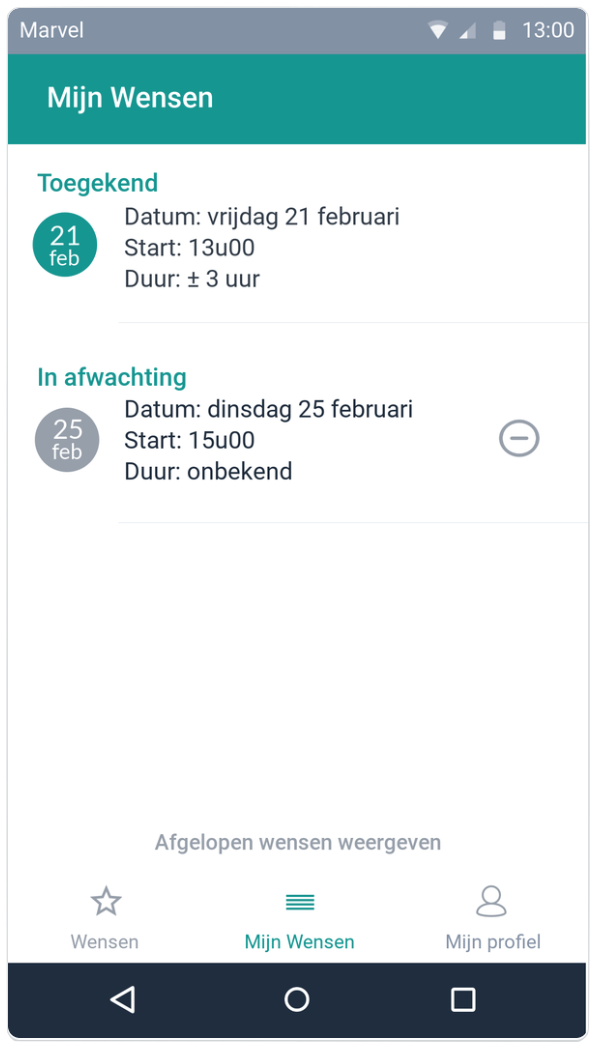
\includegraphics[width=0.76\textwidth]{care-athon/wensen.png}
  \end{subfigure}
  \begin{subfigure}[h]{0.3\textwidth}
    \centering
    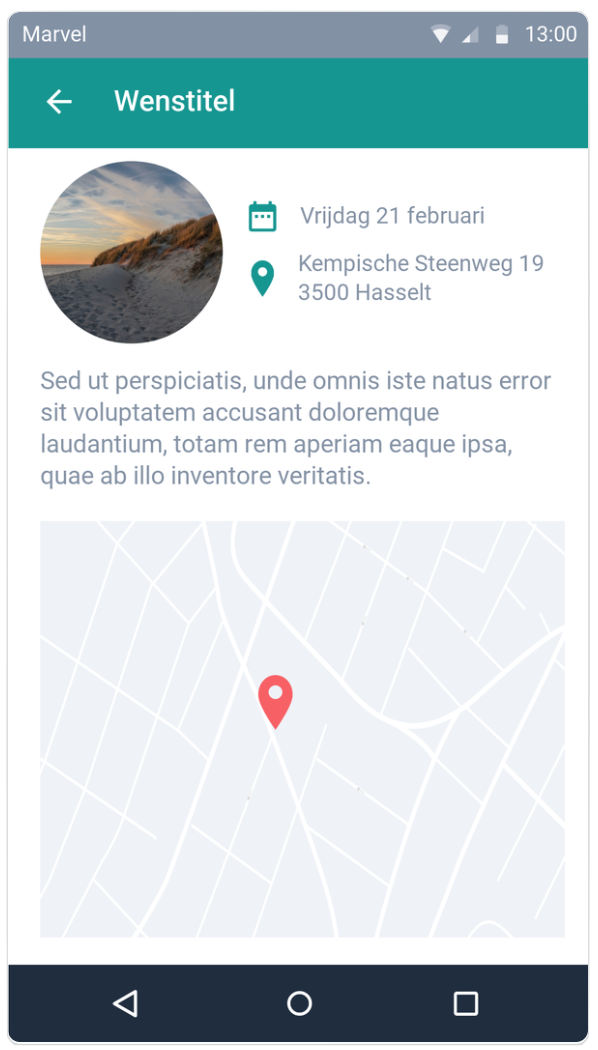
\includegraphics[width=0.76\textwidth]{care-athon/wens.png}
  \end{subfigure}
  \begin{subfigure}[h]{0.3\textwidth}
    \centering
    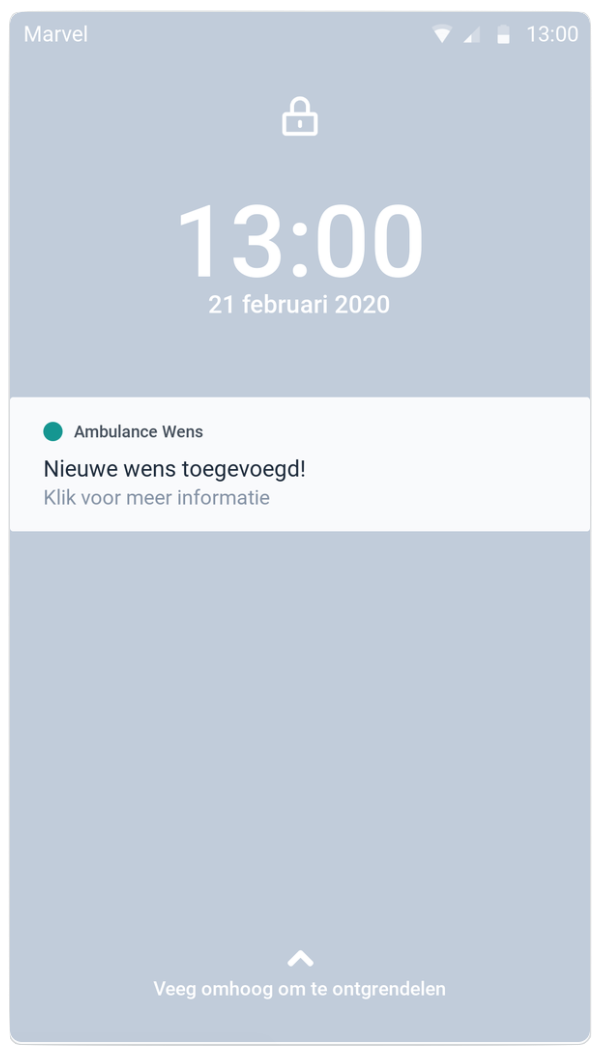
\includegraphics[width=0.76\textwidth]{care-athon/notificatie.png}
  \end{subfigure}
\end{figure}